\chapter{Problem analysis}\label{ch:ch2label}
%In today's world, programming has become an important skill \cite{ProgrammingImportant}. However, for beginners, the process of getting started with programming can be daunting due to the steep learning curve. Existing programming languages can be complex, requiring significant prior knowledge, and making it challenging for new learners to pursue programming as a career or hobby \cite{LearningCodeIsHard}.

%This problem produces an increasing demand for the creation of new programming languages that are specifically designed for beginners\cite{demandforlanguages}. These languages should be user-friendly, easy to learn, and provide an immersive experience that encourages learners to hone their skills. 

This chapter will analyze the difficulty of learning programming as a beginner programmer. It will cover some basic analysis of different programming languages with the aim of eventually comparing them, from the perspective of beginner programmers, to finally arrive at a concrete problem statement. The chapter will include facts from studies but also our own experience as beginner programmers.

\section{Learning programming }
As programming is an important skill worldwide \cite{ProgrammingImportant}, it is widely incorporated into the study curriculum of high schools and colleges. Learning text-based programming requires the student to learn, understand and remember the syntax and semantics of the language. Furthermore, the students have to evolve their computational thinking in order to solve programming problems. To learn these skills students have to be persistent in the effort of studying programming, and programming courses tend to have a high failure rate \cite{FactorsDifficultiesInProgramming}. Comparing these facts with our own experiences when being new programmers, it matches quite well. The learning curve required persistent activity and focus on the new content. \\

As an introduction to programming, block-based programming is an option. Block-based programming is mainly used to introduce children to programming, but it is also widely used in high school curricula \cite{FromBlockToText}.\\
Instead of writing lines of code and having to remember all the syntax, block-based programming is based on drag-and-drop blocks. Each block represents some function or action that the program should handle. This visual approach provides the user with an intuitive and accessible way to learn to program. The user can easily understand what they are doing and how to continue developing. Furthermore, it is quick to get easy tasks done and the user gets a visual response on what they have created \cite{FunTechBlockBased}.\\

Block-based programming has a positive impact on the motivation to learn programming and studies show that it evolves the student's computational thinking and learning of algorithmic skills \cite{FromBlockToText}. However, to continue developing as a developer, the student will reach a point where they have to switch to text-based programming.

\section{Transitioning from block-based to text-based programming} 
The use of block-based programming, in computer science educational purposes, is meant to be a preparation for the student to later transition into text-based programming languages. However, a study from 2019 states that the difficulty in learning a text-based language is not eased by first learning a block-based approach \cite{FromBlockToText}. The study investigated the learning of a text-based language in two different high school classrooms. Both classrooms followed the same curriculum but in an introductory course to programming over five weeks, they used two different versions of the same programming environment: block-based and text-based. In figure \ref{PA:pencilccFig} the two different approach is displayed. 

\begin{figure}[H] 
    \begin{center}
        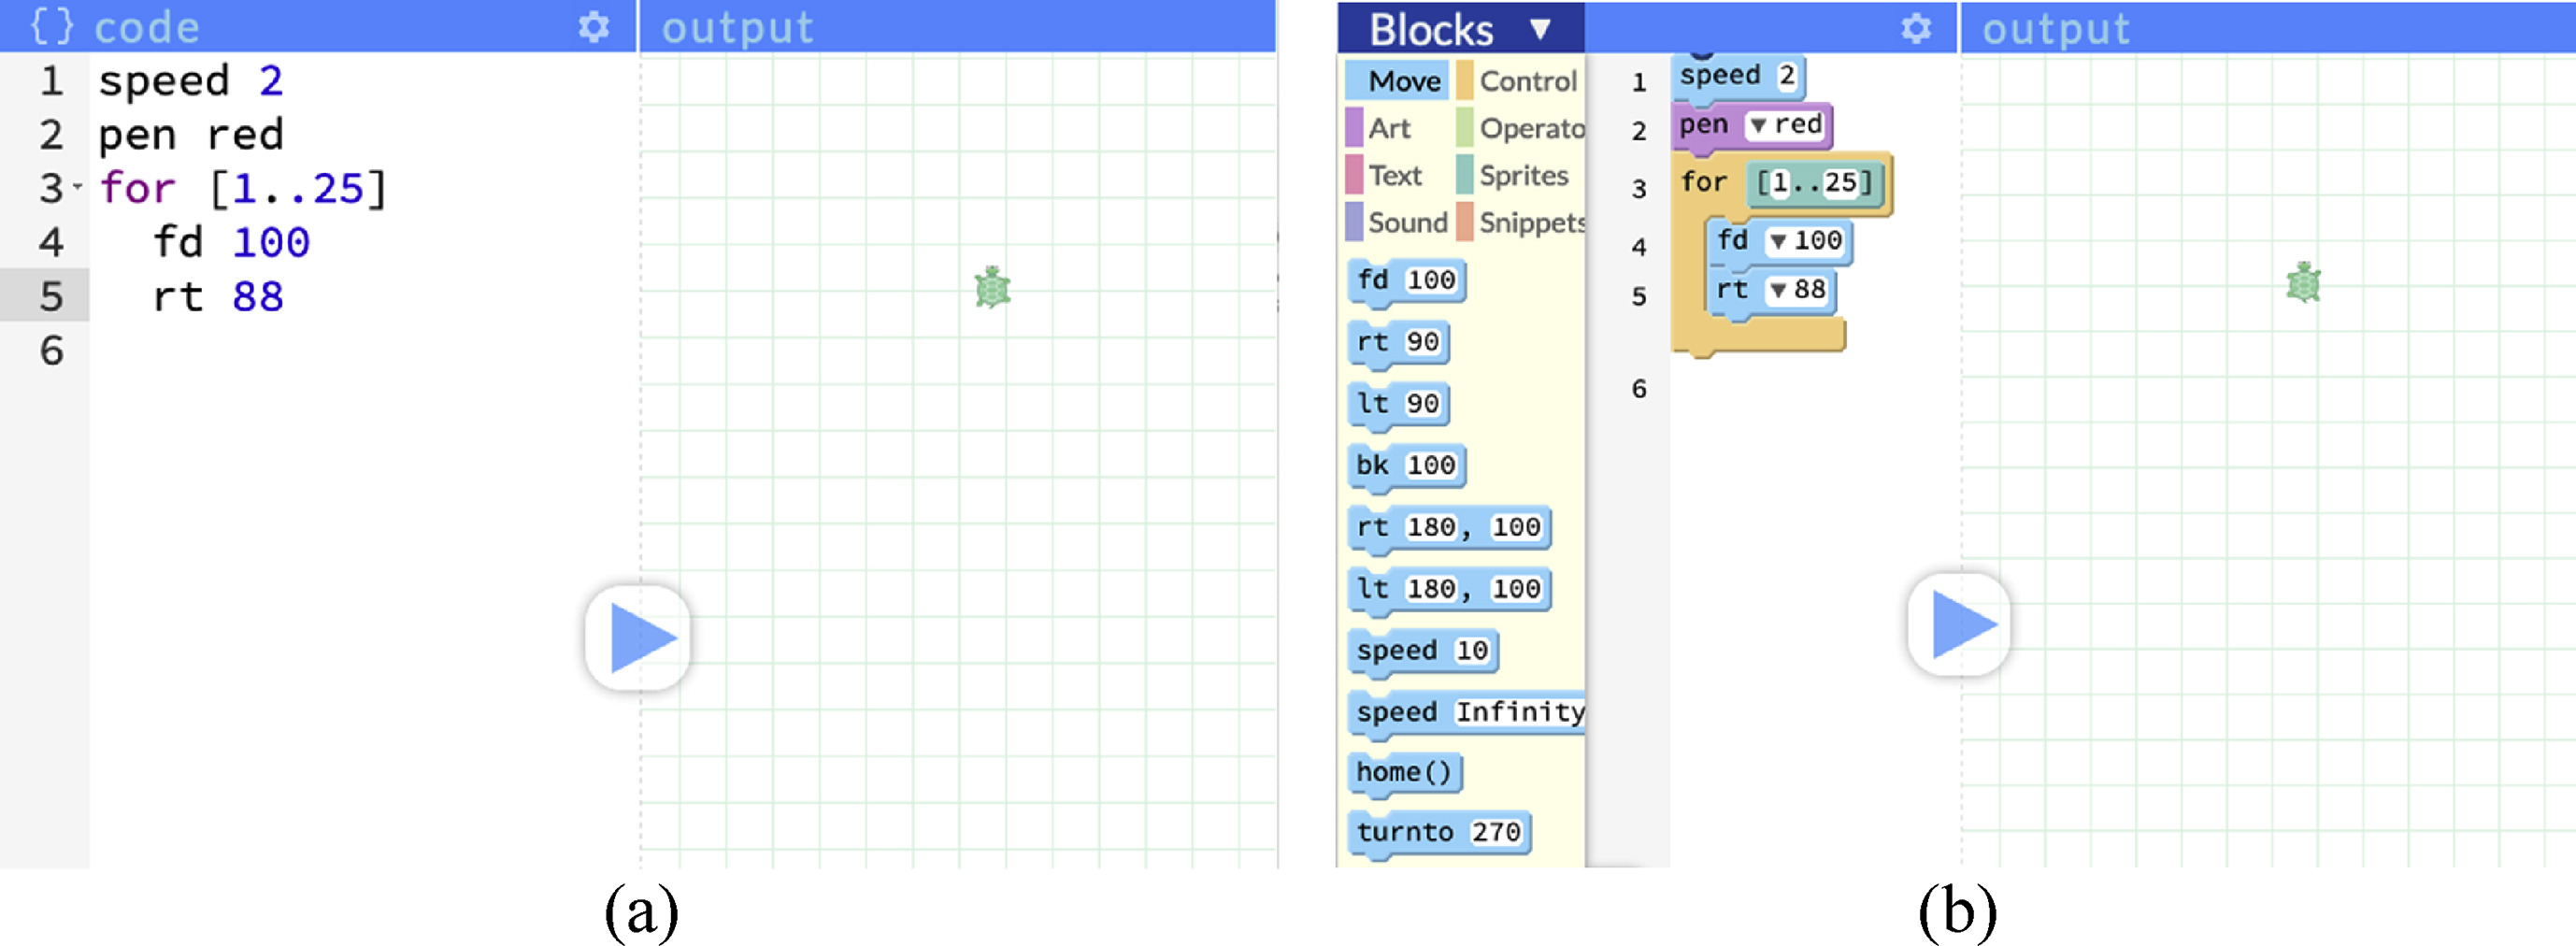
\includegraphics[width=0.9\textwidth]{Files/Billeder: Analyse/Pencilcc.jpg}
    \end{center}
    \caption{The two different approaches of the language of pencil.cc with the text-based in the left and block-based in the right \cite{FromBlockToText}.}
    \label{PA:pencilccFig}
\end{figure}

After five weeks both classes switched to learning the same text-based programming language Java. During the process, three tests were conducted, one before and after the introduction course and one after 10 weeks of learning Java. The outcome of the study is displayed in table \ref{tab:PB_A:LearningTest}. 

\begin{table}[H]
\resizebox{\textwidth}{!}{%
\begin{tabular}{|l|l|l|}
\hline
\textbf{} & \textbf{Block-based class} & \textbf{Text-based class} \\ \hline
\textbf{Test score before the learning course} & 54.3\% & 51.7\% \\ \hline
\textbf{Test score before starting the learning course} & 66.6\% & 58.8\% \\ \hline
\textbf{Test score learning Java} & 64.9\% & 65.7\% \\ \hline
\end{tabular}%
}
\caption{Overview of the average test result for the two different high school classes \cite{FromBlockToText}.}
\label{tab:PB_A:LearningTest}
\end{table}

\noindent
Table \ref{tab:PB_A:LearningTest} displays the result, it shows that the two classes were very similar in their prior programming knowledge. After the five-week introduction course, the class that followed the block-based version did significantly better. However, even though they gained a better understanding at first and scored higher on the mid-term test, the result of the last test was considered equal between the two classes. Besides the three tests that were conducted, data on their compilations were collected and reviewed. Like the test result, there was not any particular difference to find between the two classes \cite{FromBlockToText}. \\

Based on the result of the study \cite{FromBlockToText} and personal experiences of transitioning from block-based to text-based programming, using a block-based approach as an introduction to programming is simple and more intuitive for a new programmer, compared to the text-based approach. However, when switching from block-based to text-based programming, the same sense of difficulty and the same mistakes appear as for those that were introduced to programming through a text-based approach \cite{FromBlockToText}.\\

In view of the demand for new beginner programming languages, it is interesting to analyze and evaluate the differences between block-based and text-based programming. The analysis should illuminate the positive and negative aspects of text-based and block-based languages with beginner programmers as the target group.

\section{Analysis of Related Programming Languages} \label{subsection2.3}
To gain an insight into the difference between block-based and text-based languages, these will be evaluated using Sebesta's criterion, which is relevant when examining features in programming languages.\\ 

The analysis begins with the block language scratch in section \ref{section:AnalysisBlockBasesLanguages}. Furthermore, analysis and evaluation of text-based programming languages, including C, Python, and Quorum, in section \ref{text-basedlanguages}. The reasoning behind those specific languages being analyzed will be further elaborated in the following sections. \\

The languages are examined in terms of how they perform across Sebesta's criteria based on their readability, writability, and reliability. Furthermore, to identify their advantages and disadvantages for new programmers. Each criterion is further subdivided into several factors that contribute to the overall evaluation of a programming language as displayed in figure \ref{sebesta_criteria_table}. All the information upon Sebesta's criteria in this report is based on the book "Concepts of Programming languages" \cite{conceptsofproglang}. \\

\begin{figure}[H] 
    \begin{center}
        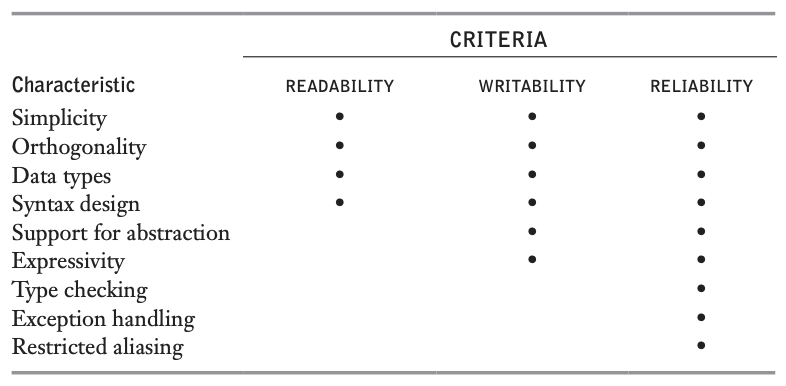
\includegraphics[width=0.9\textwidth]{Files/Billeder: Analyse/SebestaCriteria.png}
    \end{center}
    \caption{Language Evaluation Criteria and the Characteristics that affect them \cite{conceptsofproglang}.}
    \label{sebesta_criteria_table}
\end{figure}

%Figure \ref{sebesta_criteria_table} displays the three criterion: readability, writability, and reliability, and how they are effected by different factors. In the left side, the factors are listed.

\subsubsection{Readability}
Readability refers to how easy it is to read and understand code written in a particular programming language. A language that is highly readable will be easy to understand, debug, and maintain. Factors that affect readability include syntax clarity, ease of comprehension, and consistency of style \cite{conceptsofproglang}.

\subsubsection{Writability}
Writability refers to how easy it is to write code in a particular programming language. A language that is highly writable will be efficient for programmers to use, reducing development time and effort. Factors that affect writability include syntax simplicity, ease of expressing algorithms, and flexibility of control structures \cite{conceptsofproglang}.

\subsubsection{Reliability}
Reliability refers to how likely a program written in a particular programming language is to function correctly and consistently under different circumstances. A language that is highly reliable will produce fewer errors and bugs, resulting in more robust and stable programs. Factors that affect reliability include type checking, error handling, and exception handling \cite{conceptsofproglang}.

\subsection{Analysis of Scratch} \label{section:AnalysisBlockBasesLanguages}
Scratch is a Block-based programming language, which is a type of programming language that uses graphical blocks instead of traditional text-based code. These blocks represent programming concepts such as loops, conditional statements, and functions, and are typically arranged on the screen by dragging and dropping them into place. Some other popular block-based programming languages include Blockly and Code.org's App Lab \cite{popularblockbased}. Scratch is chosen because it is very popular and widely used in education, as it was developed to help children learn and express themselves through writing code. Scratch had 82 million users in December 2021, over 638 million projects created, and is the world's largest coding community for kids \cite{Scratchpopular}.\\

Scratch is a coding language with a simple visual interface \cite{scratchabout}. Scratch creates a visual environment for programmers which relies on the drag-and-drop method of programming. The different applicable components are structured in blocks with color coordination similar to LEGO blocks, as seen in figure \ref{fig:scratchexample}.\\

\begin{figure}[H] 
    \begin{center}
        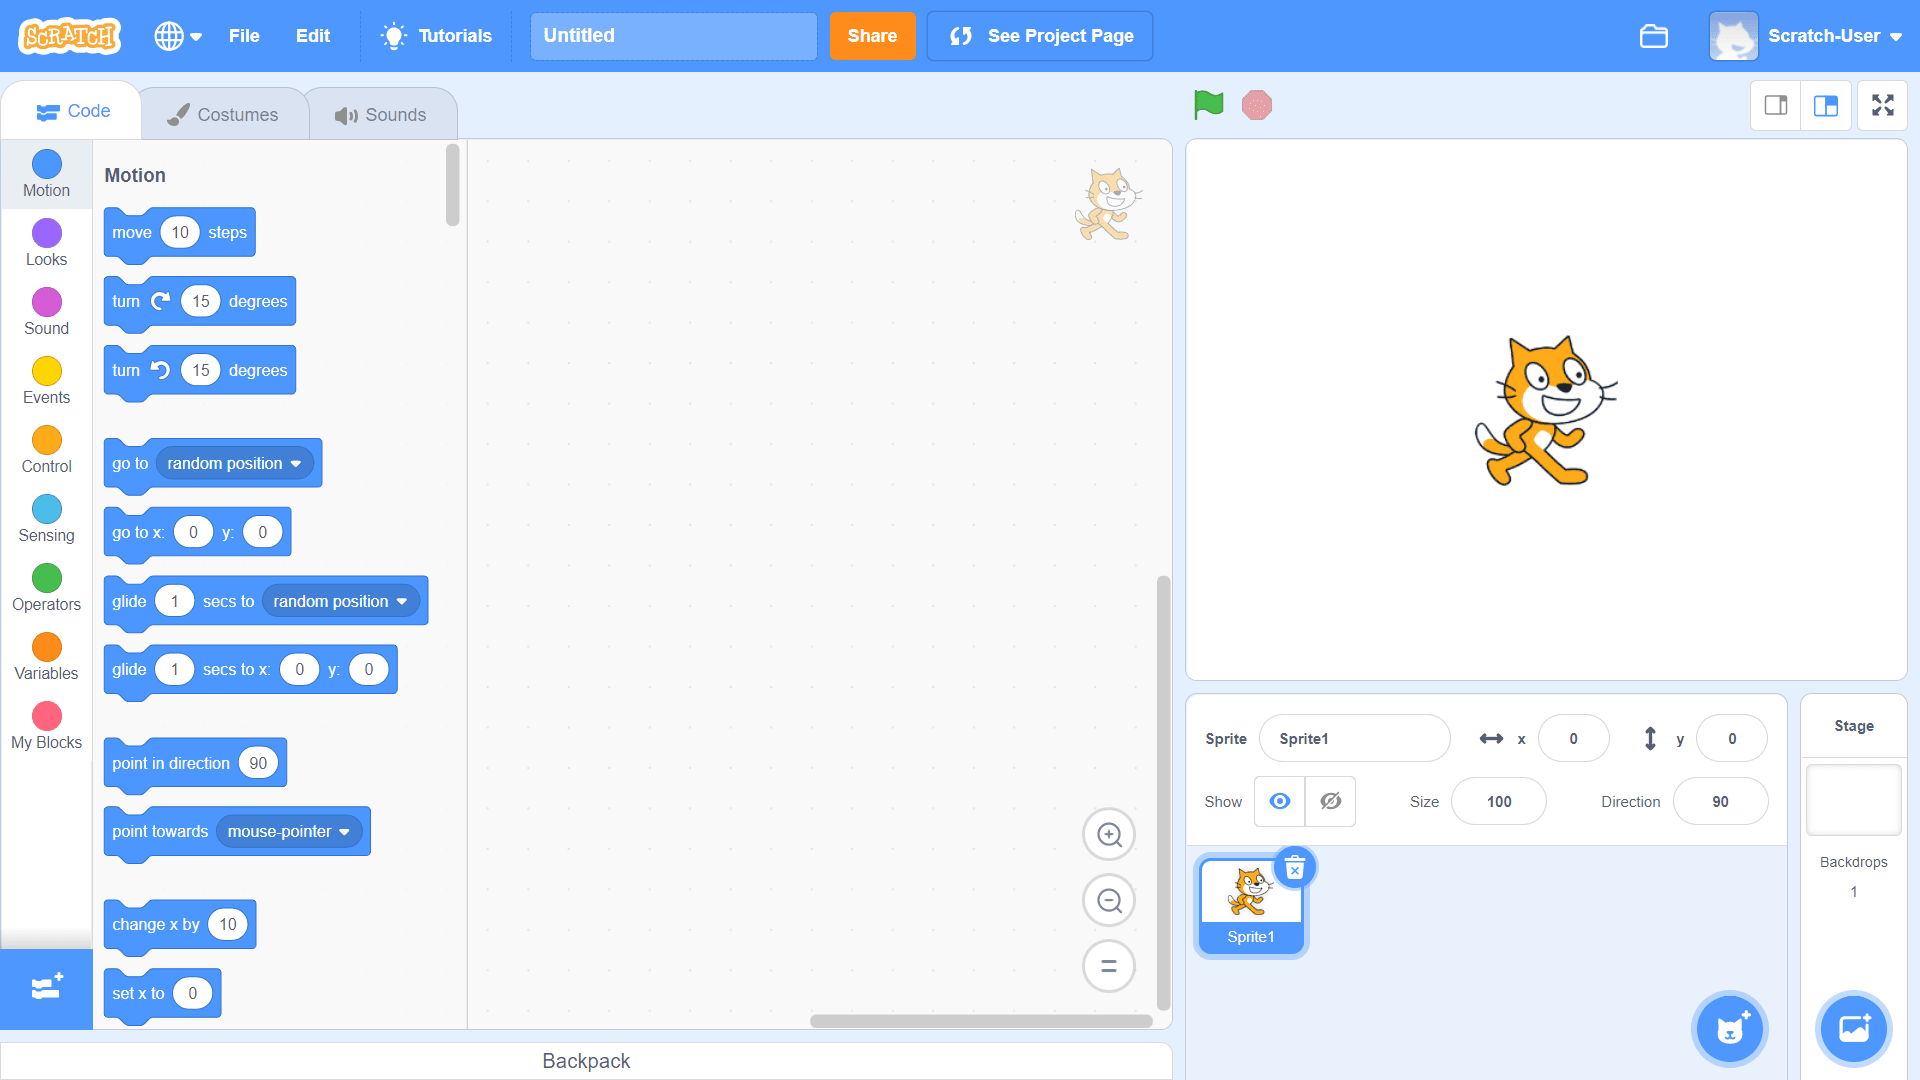
\includegraphics[width=0.9\textwidth]{Files/Billeder: Analyse/Scratch_3.0_Program.png}
    \end{center}
    \caption{Scratch Example \cite{ScratchEksempelBillede}.}
    \label{fig:scratchexample}
\end{figure}

%Blockly and code.org's App lab are similar to Scratch as they also provide a visual output of the programs as they are being developed through drag-and-drop block-based coding. They were chosen in this analysis as they are also a popular representation of the block-based programming languages \cite{popularblockbased}.

Scratch and other block-based languages, however, also have limitations in regard to their complexity. It cuts down on a lot of essential features that many of the popular text-based programming languages provide. This leads to a limited syntax, which makes it difficult to produce complex applications. The limited portability and scalability of block-based languages underline their purpose and target audience. It is clear from this that block-based languages are not intended to be widely used in the industry, but rather as a form of introduction to programming. \\

\noindent
If we take a look at Scratch in relation to Sebesta's Criteria in table \ref{sebesta_criteria_table}, the following analysis can be derived.\\

\noindent\textbf{Simplicity \& Orthogonality}\\
\noindent A language like Scratch is designed with learning in mind. Simplicity and orthogonality are very relevant when discussing block-based languages. Although Scratch is more focused on new programmers, it also has capabilities that an advanced programmer would use, including mutations of blocks or using component collections.\\

Simplicity \& Orthogonality have a special relation to mutation. A block with mutation(s) can be used in two ways. Beginner programmers can use blocks without mutations easily, while advanced users benefit from the optional parameters of the block.\\

In regards to abstract programming, component collection can be used when you want to set the width property of every button in a screen, instead of setting the property for the buttons one by one. This leads to a higher abstraction level of planning and development.\\

\noindent\textbf{Data types}\\
\noindent Scratch is very simple, and therefore only provides the basic data types such as string, number, and boolean. This also means that there are no subtypes in Scratch, such as integers or chars. This design consideration certainly simplifies the beginning phases of learning programming, since there are not multiple different ways to store a number. Still, the developer receives a core understanding of what data types are and will benefit from it if they pursue a lower-level language later on.\\

\noindent\textbf{Syntax Design}\\
\noindent The block groups have different colors and it is possible to play with the shapes of the blocks related to their different stacking and embedding types. This means that each block can contain different kinds of function block shapes e.g. a number that is a rectangle with rounded corners fits inside a "change x by *shape*" command block. These methods are very helpful for beginners in developing programs since they are given clues as to how to stack the blocks on top of each other. This usually benefits syntax considerations and avoids irritating "syntax error" messages.\\

\noindent\textbf{Support for abstraction}\\
Scratch has limited support for abstraction in the form of function definition. The programmer is able to create their own blocks and manipulate them to an extent. However, generalization of data types is not possible and it can be argued that the functions which can be created are restricted in their complexity. \\
% Most block-based languages are intended to support process abstraction, but it is also possible to find some data abstraction support, e.g. colors. Process abstraction is very important in block languages and the development method depends on the level of abstraction.\\


%What this means is that a higher level of process abstraction is a help for the beginner. As is the language, which is simple up to a specific level, since too many abstract processes could be confusing for a beginner.\\

\noindent\textbf{Expressivity}\\
\noindent Expressivity in Scratch is enhanced by the presence of powerful blocks that make it possible to accomplish a lot with a few blocks. This does mean that the programmer does not have full freedom in using these blocks, however, they do accelerate the learning process for beginners as they move towards the intermediate level. Apart from this, Scratch provides limited expressivity, as there in most cases are not multiple ways of accomplishing the same task. This is due to the blocks being specialized for specific purposes, taking away some freedom from the programmer while simplifying their use.\\

\noindent\textbf{Type checking}\\
\noindent 
Scratch performs type-checking to ensure that the blocks used in a script are compatible. In Scratch, the blocks are geometrically shaped to indicate their types, like in figure \ref{fig:scratchblocks}. For example, a boolean is shaped like a hexagon, and a rounded rectangle is for numbers or strings. By using these shapes, you are able to look at command blocks and the shapes they accept, to determine which kind of types you should make use of. This version of type-checking allows beginners to understand that there exist different types, which are not all interchangeable \cite{Scratchblocks}.

\begin{figure}[H]
    \begin{center}
        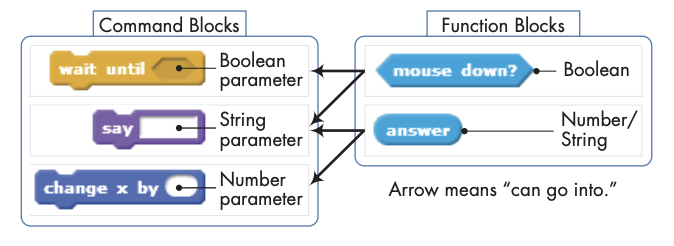
\includegraphics[width=0.75\textwidth]{Files/Billeder: Analyse/Scratchblocks.png}
    \end{center}
    \caption{Scratch blocks \& types \cite{Scratchblocks}.}
    \label{fig:scratchblocks}
\end{figure}

\noindent\textbf{Exception handling}\\
\noindent Exception handling is not usually an accessible feature of Block-based languages. There are no known statements on why exception handling is not an implemented feature within most block-based languages. However, it is fair to say Exception handling can be a complex concept for beginner programmers \cite{exceptionhandling}, and could therefore be the reason why it is not implemented. This means Scratch programs simply have to be error-free in order to run without crashing.\\

\newpage
\noindent\textbf{Restricted aliasing}\\
\noindent Since you are not able to have two or more distinct names in a block-based language that can access the same memory cell, as well as the lack of pointer implementation or a form of reference, Scratch does not have aliasing, and strict aliasing is not a relevant problem.\\

\noindent\textbf{Summary}\\
\noindent Block-based programming languages rely on graphical blocks instead of traditional text-based code, with Scratch being one of the most popular, with 82 million users and over 638 million projects created. Other popular block-based programming languages include Blockly and Code.org's App Lab. The simplicity and orthogonality of Scratch make it an excellent language for new programmers to learn. However, this simplicity also means Scratch is limited in terms of complexity, making it difficult to produce complex applications. The text also provides an analysis of Scratch in relation to Sebesta's Evaluation Criteria, discussing its simplicity, data types, syntax design, support for abstraction, and expressivity. Overall, Scratch is an excellent language for teaching basic coding concepts to children and beginners, but may not be suitable for developing more advanced applications.

\subsection{Analysis of relevant text-based programming languages} \label{text-basedlanguages}
%Widely used in the industry
%Beginner friendly (Often used by beginners)
%A "hard", widely used language, in order to compare the differences between easy and hard
%Quorum has been chosen because it is evidence based, and also focuses on teaching programming.

%A relevant language, in this case, is defined as a language often used by beginners as their introductory language, or a language widely used in the industry. 

In section \ref{SelectionLang}, three text-based programming languages are analyzed. In order to select more relevant languages to analyze, considering programming paradigms is appropriate.

\subsubsection{Programming Paradigms}
Programming paradigms help categorize different styles of programming and can be used to describe a programming language. Some of the most commonly used programming paradigms include 'imperative' and 'declarative'. The imperative programming paradigm is a way of programming where the instructions given are used to change between states. Each instruction given, like changing the contents of a variable, represents a state change \cite{WikiProgrammingParadigms}. Examples of this are C, Java, and C\#. \\
In the declarative programming paradigm, no instructions regarding how to compute anything are given, rather the properties of the needed result are given and the underlying required computations are made based on this result \cite{WikiProgrammingParadigms}. Examples of this are most database query languages like SQL. Because many paradigms are similar and/or derive from other paradigms, most programming languages are considered to be multi-paradigms.\\ 

\newpage \noindent
\textbf{Procedural programming:} Within the imperative- and declarative programming paradigm are subcategories. Both 'procedural' and 'object-oriented' are subcategories of imperative programming. The procedural paradigm is about changing states using procedures/subroutines. Procedures are functions with the purpose of changing the value of their arguments and they do not return an output. Most procedural languages are also imperative but the main difference is that the procedural paradigm depends on scopes and therefore most languages containing control structures like \textit{for}, \textit{while} and \textit{if} are procedural \cite{WikiProgrammingParadigms}. A language without scopes that instead use for example 'goto' would be considered imperative but not procedural. C, Java, and C\# are also considered procedural programming languages. \\
%https://en.wikipedia.org/wiki/Procedural_programming

\noindent
\textbf{Object-oriented programming:} Instead of changing states through procedures, the object-oriented paradigm changes states through its objects which themselves can contain procedures and functions. In this way, they are similar to the procedural paradigm, and usually, an object-oriented programming language is also considered procedural as it supports procedures and sequences of instructions \cite{WikiProgrammingParadigms}. Examples include Java and C\#. \\
%https://en.wikipedia.org/wiki/Procedural_programming

\noindent
\textbf{Functional programming:} The most notable subcategory within declarative programming is functional programming. In functional programming, the result wanted by the user is defined using a series of functions \cite{FunctionalProgrammingParadigm}. In the functional paradigm, a function cannot contain side effects, meaning that any input is mapped directly to an output. There do not exist popular purely functional programming languages, though some languages like C\# include features from the functional paradigm with their use of LINQ and lambda expressions \cite{FunctionalProgrammingParadigm}. \\
%https://en.wikipedia.org/wiki/Functional_programming

\subsection{Selecting the languages} \label{SelectionLang}
The languages will be from the imperative programming paradigm, including the paradigms: procedural and Object-oriented, as languages in these paradigms, are easy to learn and read, compared to languages from the declarative paradigm \cite{ProgrammingParadigme}.\\

When considering the selection of languages to analyze within the imperative paradigm, Python, Quorum, and C is chosen based on the following arguments:

Python is chosen because it has a simple syntax \cite{PythonLanguageReference}, is widely used in the industry \cite{TopProgrammingLanguages2022}, and is a common starting language for new programmers \cite{PythonBeginnerProgrammingLanguage}. \\

Quorum is interesting to analyze because it is used as an introductory language, e.g. in high schools. It has a simple and readable language design \cite{QuorumVid}. Furthermore, Quorum is an evidence-based language meaning that it was developed based on the results of scientific research in order to improve its language design \cite{QuorumProgLang}.\\

C is selected because it is widely used in the industry \cite{5ReasonsForC}, and because it is the predecessor for many other widely used languages such as Python, Java, and C\#. This can be seen in figure \ref{Prog_Lang_Tree}. C and Python are circled to indicate their presence in the tree, and the red lines indicate the connection between C and the other mentioned languages. However, C is viewed as a less beginner-friendly language, as it has constructs such as pointers, dynamic memory allocation, etc, which can be hard to grasp for new programmers \cite{5ReasonsForC}. 

\begin{figure}[H] 
    \begin{center}
        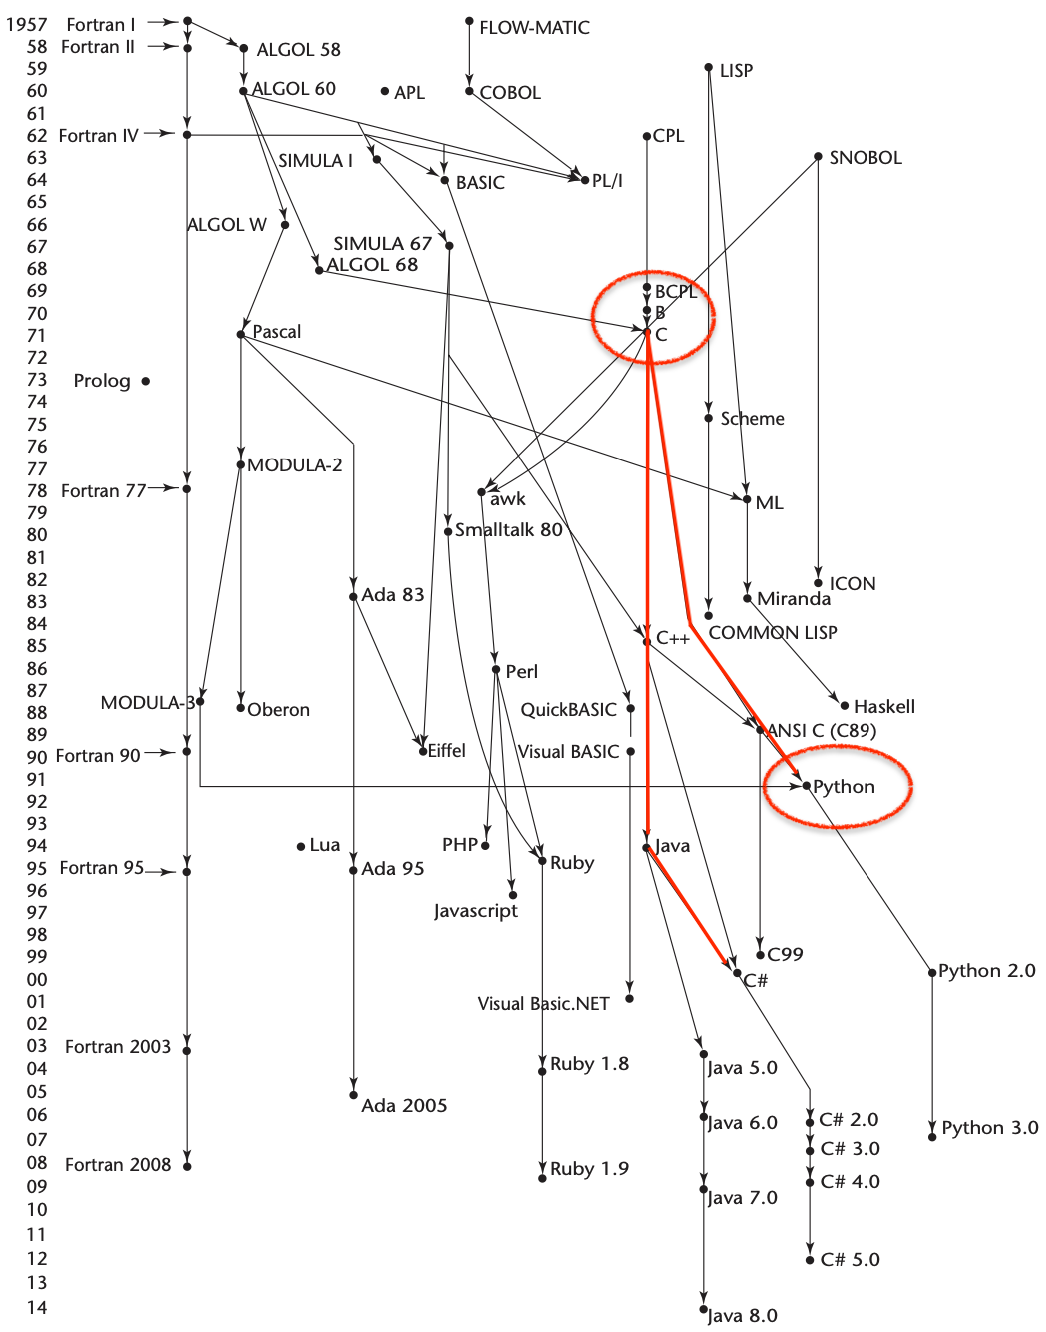
\includegraphics[width=0.9\textwidth]{Files/Billeder: Analyse/ProgTree.png}
    \end{center}
    \caption{A programming language evolution tree. \cite{conceptsofproglang}.}
    \label{Prog_Lang_Tree}
\end{figure}

\newpage
\subsubsection{Python Language}
Python is an object-oriented programming language with a simple syntax. Python supports multiple programming paradigms such as procedural and functional programming \cite{PythonLanguageReference}. The Python programming language is considered a high-level text-based programming language. With an easy and English-like syntax, Python is considered a beginner-friendly language \cite{PythonGoodForBegin}. An example of a small Python program can be seen in figure \ref{codeEx:Python}\\

\begin{figure}[H] 
    \begin{center}
        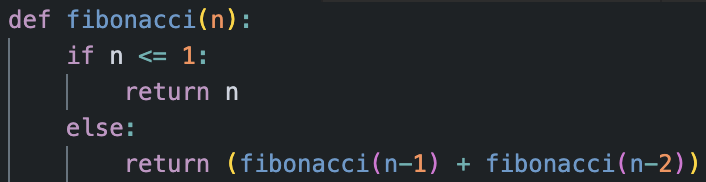
\includegraphics[width=0.9\textwidth]{Files/Billeder: Analyse/PythonFiboExample.png}
    \end{center}
    \caption{Python Fibonacci Example.}
    \label{codeEx:Python}
\end{figure}

\noindent\textbf{Simplicity}\\
\noindent In Python few lines can amount to larger functionalities. Due to this, some concepts can be easy to learn and read while others can seem cryptic. Python's short syntax makes it easier to write code, improving writability overall.\\

\noindent\textbf{Orthogonality}\\
\noindent Python has a high degree of orthogonality. This means that the constructs in the language can be combined in multiple ways which initially makes Python easier to read and write \cite{progEvalArticle}. However, having very high orthogonality might be a disadvantage, as it then allows very complex constructs due to combinatorial freedom.
\\

\noindent\textbf{Data types}\\
\noindent Python has multiple built-in data types, such as integers, strings, and floats, but it also supports more complex data types such as lists, etc. With many built-in data types, expressivity is improved. However, there are some downsides to having a lot of built-in data types, one of which is making the language more complex and harder to learn.\\

\noindent\textbf{Syntax design}\\
\noindent Pythons syntax is short and readable \cite{PyntaxSyntax}, which helps improve readability and writability. Python syntax uses indentation instead of curly brackets as scopes, which for some users makes the code more readable, whereas it can cause confusion for others who are used to curly brackets.\\

\noindent\textbf{Support for abstraction}\\
\noindent Python includes support for abstraction by letting the programmers define their own functions and classes and such. By having support for abstraction, writability is increased as it allows some functionality to be reused later on.\\

\noindent\textbf{Expressivity}\\
\noindent Python has high expressivity. This is due to the fact that Python allows its programmers to express ideas in multiple different ways, each with their own advantages. Expressivity can improve readability and writability. However, high expressivity may also make the language harder to read for some, as too many ways of expressing the same functionality may cause confusion. The programmer has to keep track of a larger collection of constructs in order to fully utilize the functionality of the language.\\

\noindent\textbf{Type checking}\\
\noindent Python is a dynamically typed language, which means that the interpreter assigns variables a type at runtime based on the variable's value at the time \cite{Dynamic_Typing}. By being a dynamically typed language Python becomes more flexible. It can also lead to some type-related errors which may be difficult to catch during development. However, Python is at the same time strongly typed, meaning that variables have a type and that it matters when performing operations on the variable.\\

\noindent\textbf{Exception handling}\\
\noindent Python has support for exception handling. This makes it easier to develop code that can handle errors, which can help improve reliability by handling errors, which are expected to occur.\\

\noindent\textbf{Restricted aliasing}\\
\noindent Python does not have restricted aliasing. This slightly lowers the reliability of the language compared to languages that support it.

% Python has restricted aliasing. This improves reliability by having some unexpected changes due to changes to some of the shared data that can happen with aliasing.\\


\noindent\subsubsection{Quorum Language}
\noindent Quorum is a high-level programming language, which is intended mainly for students but is broad enough to also be used commercially \cite{QuorumProgLang}. One of the main focuses of the language is for its syntax to be simple and accessible because it is meant to be easy to learn for all types of learners. Furthermore, it aims to improve language design overall \cite{QuorumVid}. An example of a small Quorum program can be seen in figure \ref{codeEx:Quorum}\\

\begin{figure}[H] 
    \begin{center}
        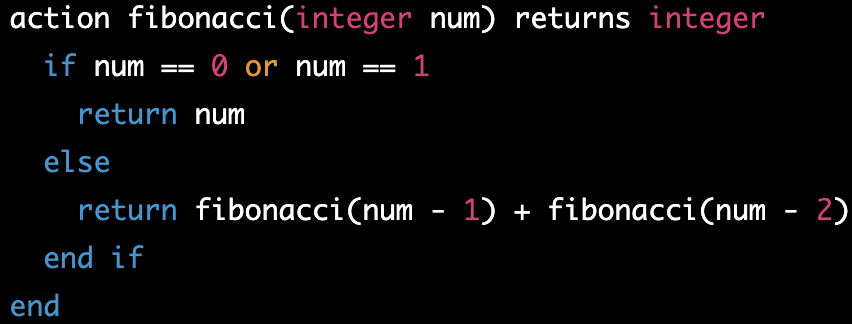
\includegraphics[width=0.9\textwidth]{Files/Billeder: Analyse/QuorumFiboExample.png}
    \end{center}
    \caption{Quorum Fibonacci Example.}
    \label{codeEx:Quorum}
\end{figure}

\noindent\textbf{Simplicity}\\
\noindent Since quorum is designed to be simple and easy to learn, its syntax is straightforward and easy to read, which enhances its readability. Its simplicity also enhances the language's writability. Finally, Quorum's simple design helps to reduce the potential for errors, which enhances its reliability.\\

\noindent\textbf{Orthogonality}\\
\noindent Quorum supports a relatively small set of primitive constructs that can be combined in a variety of ways to build control and data structures. This orthogonality helps to make the language easy to learn and use, which enhances readability and writability. Additionally, orthogonality increases the reliability of code written in the language.\\

\noindent\textbf{Data types}\\
\noindent The data types supported by Quorum include integers, booleans, strings, and arrays. The use of clear and consistent data types enhances Quorum's readability and writability, as it is easy to understand the purpose and behavior of different data types. Furthermore, the use of strong typing and type-checking mechanisms helps to improve the reliability of code written in the language.\\

\noindent\textbf{Syntax design}\\
\noindent Quorum's syntax is designed to be simple and clear, which enhances its readability. The use of consistent and intuitive syntax design also helps to improve the language's writability, as developers can easily understand how to use different language constructs. However, writability is not as high as it could be, since the syntax in many cases, forces the developer to write the full name of a construct, e.g. "boolean", instead of "bool", as booleans are called in some programming languages. Having to write the full-length construct names instead of an abbreviation, increases readability, but reduces writability, as the programmer would be able to write a program faster using abbreviations for the constructs. Finally, the use of a clear syntax design improves the reliability of code written in the language.\\

\noindent\textbf{Support for abstraction}\\
\noindent Quorum includes support for abstraction, in the form of object-oriented features such as inheritance and encapsulation. This helps improve writability and reliability, as the developer is able to write reusable code that is easy to modify and maintain.\\

\noindent\textbf{Expressivity}\\
\noindent Quorum low expressivity as it does not have many ways of expressing the same computations. For example, the count++ notation from C and other languages does not exist in Quorum, where the only way of counting up a variable is "count = count + 1". An example where Quorum contains constructs that can specify the same computation is with its loops. Quorum has three types of loops: Repeat x times, repeat until, and repeat while. Repeating x times makes it easy to repeat the same action a specific amount of times. However, repeat until and repeat while can also be used for the same purpose, but are more powerful, as they both run based on a boolean condition. By itself, the quorum language does not have very high expressivity, however, this changes with its different libraries, which simplify many different actions. Expressivity enhances the language's readability and writability, and developers can use language constructs that are intuitive and easy to understand.\\

\noindent\textbf{Type checking}\\
\noindent Quorum is statically typed and includes strong type-checking mechanisms, which help to improve the reliability of code written in it. Type checking helps to ensure that code is correct and free from errors related to data types.\\ 


\noindent\textbf{Exception handling}\\
\noindent Quorum includes support for exception handling by the programmer, which helps to improve the reliability of code written in the language. The error handling in Quorum allows the use of a Try-Catch-Finally statement, however, the syntax is different, as Quorum uses a check-detect-always syntax instead. \\


\noindent \textbf{Restricted aliasing}\\
\noindent Quorum does not include support for restricted aliasing, which slightly lowers the reliability of the language compared to languages that support it.
% Quorum includes support for restricted aliasing, which helps to prevent errors related to data aliasing. This enhances the language's reliability, as it helps to prevent errors that can be difficult to detect. \\


\subsubsection{C Language}
C is an imperative text-based programming language that is considered low-level compared to other more popular languages like Python or C\#\cite{WikiCLang}. It is widely used due to its lower level, making it an efficient language for writing code closely linked to machine instructions. One way that C is considered low level is for example its inclusion of pointers, which can point to an address in memory, similarly to machine instructions in assembly\cite{WikiCLang}. An example of a small C program can be seen in figure \ref{codeEx:C}
%https://en.wikipedia.org/wiki/C_(programming_language)

\begin{figure}[H] 
    \begin{center}
        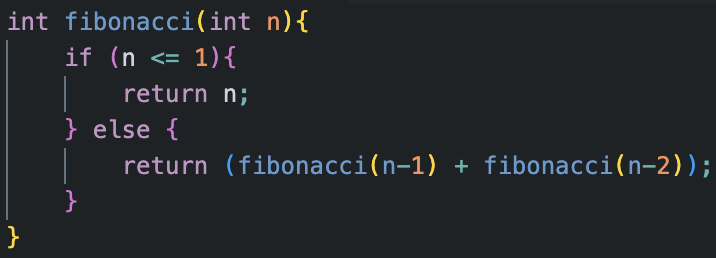
\includegraphics[width=0.75\textwidth]{Files/Billeder: Analyse/CFiboExample.png}
    \end{center}
    \caption{C Fibonacci Example.}
    \label{codeEx:C}
\end{figure}


\noindent\textbf{Simplicity}\\
\noindent C has a limited amount of data types and keywords making it simple, however, some instructions, which in other languages require one line, may require multiple lines in C. An example of this is C's lack of built-in properties like arrays ".length" property which exists in most languages. An arrays length can be accessed any time through the array in C\# and Python, while in c you would have to initialize the array and calculate the length of the array on separate lines. The language also requires some knowledge of low-level programming because of its inclusion of concepts like pointers and dynamic memory allocation. \\

\noindent\textbf{Orthogonality}\\
\noindent C does not include higher-level components such as lists, but combining the components that are included can create more advanced structures. In C, certain operators cannot be used on some data types which are otherwise possible in some higher-level languages like C\#. For example in C strings cannot be concatenated using "+".\\

\noindent\textbf{Data types}\\
\noindent In C there are a limited amount of data types. Today most languages include data types like "bool" and "string". In C, "true" is represented by any integer value that is not 0, and to make a string, an array of characters is needed. \\

\noindent\textbf{Syntax Design}\\
\noindent Some of the syntax in C can be considered hard to learn for beginners such as pointers and indirect component selection of struct fields. Many words are reserved and have special meanings in C. The only keyword which violates this is the keyword "static" which can be used to declare global variables within a scope, or used to define that an array parameter needs a specific length.\\

\noindent\textbf{Support for Abstraction}\\
\noindent In C, the programmer is able to create abstraction by using functions and structs. These abstractions can be considered low compared to higher-level languages which include classes, inheritance, and dynamic objects.\\

\noindent\textbf{Expressivity}\\
\noindent In higher-level languages the programmer is able to have more functionality on fewer lines than in C. Despite this, code can be written concisely in C though it may be hard to read.\\

\noindent\textbf{Type Checking}\\
\noindent C contains limited methods of type checking. C allows implicit typing, making detecting errors difficult\\

\noindent\textbf{Exception Handling}\\
\noindent C does not have built-in exception handling like other higher-level languages. For example, Quorum and Python have a try-catch structure and the ability to throw an error, like previously mentioned in their analysis. "Try-catch" and throwing an error is not possible in C\\

\noindent\textbf{Restricted aliasing}\\
\noindent C has "restricted pointers" which helps express anti-aliasing in C but besides this, C's heavy need for pointers when making functionality, makes aliasing occur often in the language. The restrict keyword on a pointer is a way of telling the compiler that the specific pointer is the only way of accessing the object pointed by it \\

\subsection{Comparing languages} \label{ComparingLanguages}
In this section, a comparison between the languages previously analyzed in section \ref{subsection2.3} is conducted. These languages will be compared based on their overall readability, writability, and reliability in order to understand the difference and deduct how a language aimed at beginners, compares to these languages. Each language is put on a scale ranging from low to high on readability, writability, and reliability. These scales represent how these language rank compared to each other based on the analysis.

\newpage
\subsubsection{Comparing readability}
First up is comparing readability. The languages are ranked on the scale,  displayed in figure \ref{PA:readability_scale}. 

\begin{figure}[H] 
    \begin{center}
        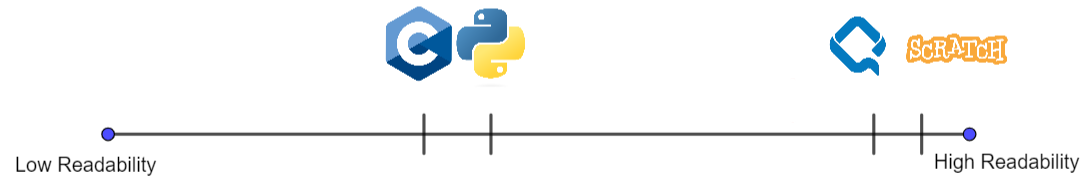
\includegraphics[width=0.9\textwidth]{Files/Billeder: Analyse/Readability.png}
    \end{center}
    \caption{The programming languages C, Python, Quorum, and Scratch placed on a scale showing readability.}
    \label{PA:readability_scale}
\end{figure}

C has the lowest readability of the languages that have been analyzed in figure \ref{PA:readability_scale}. This is due to the fact that it is a low-level programming language, in which a line of code often closely resembles machine instructions. The main reason for not placing C lower on the readability scale is due to the fact that languages such as Assembly have notably lower readability. \\

Next on the scale in figure \ref{PA:readability_scale} is Python which has better readability. The reason is that Python focuses a lot more on writability which will be elaborated on in figure \ref{PA:writability_scale}. In Python, the programmer is able to write readable code for intermediate programmers while also having the ability to write a lot of functionality within a few lines which may be confusing for beginner programmers.\\

The next language on the scale in figure \ref{PA:readability_scale} is Quorum. Quorum has been placed high on the readability scale. This is due to the fact that Quorum has a simple syntax, which focuses on readability over writability. Compared to a language like Python where the programmer is able to write flexible code with a focus on writability and less readability, there is less room for complex code in Quorum as it focuses on simplicity.\\

Scratch has high simplicity which makes it more beginner friendly and readable. Every block is labeled in order to remove ambiguity in the language (see figure \ref{fig:scratchexample}). Coding larger functionalities in Scratch could be considered confusing for beginners, due to the large amount of blocks which can be combined, but despite this, the blocks still help define the functionalities.\\

\subsubsection{Comparing writability}
Next, is comparing the writability. The languages is ranked on the scale,  displayed in figure \ref{PA:readability_scale}. 

\begin{figure}[H] 
    \begin{center}
        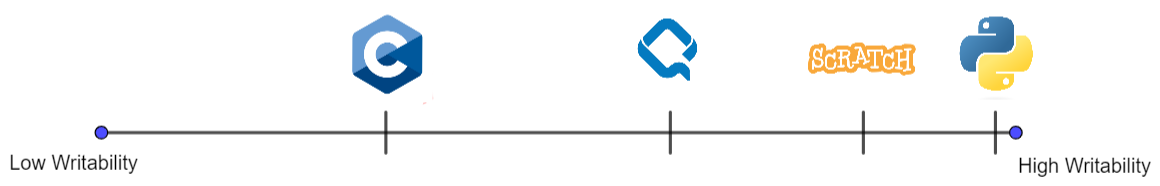
\includegraphics[width=0.9\textwidth]{Files/Billeder: Analyse/Writability.png}
    \end{center}
    \caption{The programming languages C, Python, Quorum, and Scratch placed on a scale showing writability.}
    \label{PA:writability_scale}
\end{figure}

The language with the lowest writability on the scale in figure \ref{PA:writability_scale} is C. One of the reasons for this is due to C being a low-level language and therefore has low expressivity. C does not contain many ways in which you can express complex concepts in a few lines. Compared to higher-level languages, C also has less support for abstraction like previously mentioned in the analysis. In general, C is very bare-bones and limited compared to other languages.\\

Quorum is placed in the on figure \ref{PA:writability_scale} regarding writability. Compared to C, it is more expressive and has more support for abstraction, for example in the form of its object-oriented features. Quorum is placed lower compared to Python and Scratch because of its need to be readable. For example, the data type "int" in C, is an abbreviation for "integer", which is the name used in Quorum.\\

In Scratch, each "block of code" has to be dragged in. This makes it simple to create code since all available code blocks can be seen in a sidebar. Scratch is placed lower on figure \ref{PA:writability_scale} than Python because despite how easy this is, Scratch has limited expressivity compared to Python where it may be faster to write code than looking for and dragging in multiple blocks.\\

Especially because of Python's high level of expressivity, a lot of functionality can be written in a few lines. Python is therefore placed highest on the scale in figure \ref{PA:writability_scale}. Python also has a lot of support for abstraction and orthogonality compared to C, Quorum, and Scratch.\\

\newpage
\subsubsection{Comparing reliability}
The last criterion that is compared is reliability. The languages are ranked and displayed in figure \ref{PA:reliability_scale}.

\begin{figure}[H] 
    \begin{center}
        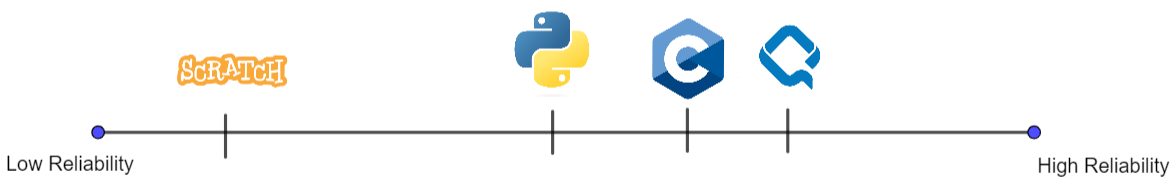
\includegraphics[width=0.9\textwidth]{Files/Billeder: Analyse/Reliability.png}
    \end{center}
    \caption{The programming languages C, Python, Quorum, and Scratch placed on a scale showing reliability.}
    \label{PA:reliability_scale}
\end{figure}

Scratch does not have exception handling and is dynamically typed. If the programmer decides to set the value of a variable equal to two strings added together, no error is displayed, and instead, the value becomes 0. This makes Scratch less reliable and Scratch is therefore placed lowest on the scale in figure \ref{PA:reliability_scale}, as the programmer is not warned about unwanted behavior. Scratch does have restricted aliasing making it slightly more reliable.\\

Python is dynamically and strongly typed and is able to for example interpret strings to numbers and vice versa, however, the programmer can get unwanted behavior when letting Python do automatic type conversion. Python still allows for explicit type conversion though. This gives Python lower reliability, ranked lower than C and Quorum on the scale in figure \ref{PA:reliability_scale}, but higher reliability than Scratch.\\

In C the programmer does not have access to exception handling, but C is statically typed making it more reliable than Python and Scratch in figure \ref{PA:reliability_scale}. C has limited support for restricted aliasing, but with its focus on using pointers, it does have aliasing.\\

Quorum provides exception handling for the programmer and is statically typed. This makes Quorum more reliable than the other languages analyzed. 

\begin{comment}
\subsection{Comparing languages}
In this section, a comparison between the languages previously analyzed in section \ref{subsection2.3} is made. These languages will be compared based on their overall readability, writability, and reliability in order to understand the difference and deduct where a language aimed at beginners, lies on the scales compared to other languages. The goal for the language is to be readable and understandable for beginners while also making the transition to other industry standards easier. Therefore the goal is to prioritize readability higher than writability while also making sure that it is somewhat reliable.

\subsubsection{Comparing readability}
The first language on the scale is C. C has the lowest readability of all the languages which have been analyzed. This is due to the fact that it is a low-level programming language, in which a line of code often closely resembles machine instructions. \\

Next on the scale is Python which has better readability. The reason is that Python focuses a lot better on writability which will be elaborated on in figure \ref{writability}. In Python, the programmer is able to write readable code while also having the ability to write a lot of functionality within a few lines which may be considered unreadable.\\

The next language on the scale is Quorum. Quorum has been placed high on the readability scale. This is due to the fact that Quorum has a simple syntax, which focuses on readability over writability. Compared to a language like Python where the programmer is able to write flexible code with a focus on writability and less readability, there is less room for complex code in Quorum as it focuses on simplicity.\\

Scratch has high simplicity which makes them more beginner friendly and readable. Every block is labeled in order to remove ambiguity in the language. Coding larger functionalities in Scratch could be considered confusing due to the large combination of blocks, but despite this, the blocks still help define the scopes clearly and concisely.\\

After analyzing these languages, and making some considerations about where on the scale, the language \lang should be placed, it has been decided that \lang should be very readable in order to help beginners. However, at the same time, it should also help new programmers with transitioning to some common industry standards. Because of this, \lang has been placed between Python and Quorum, but closer to Quorum. This is due to the focus on readability, as people who have not programmed before, should be able to recognize the constructs of \lang. This would help beginners learn the language quicker as well. Figure \ref{readability} visualizes a comparison of the language's readability on a simple scale. To simplify, block-based languages are represented by the Scratch programming language

\begin{figure}[H] 
    \begin{center}
        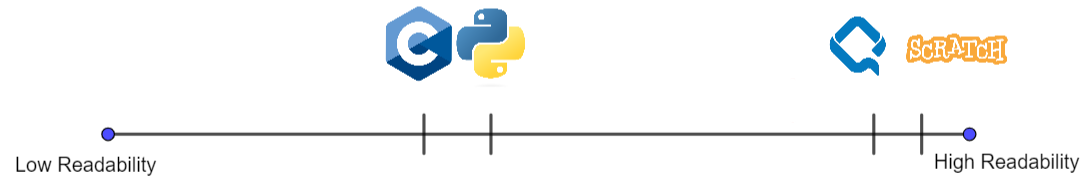
\includegraphics[width=0.9\textwidth]{Files/Billeder: Analyse/Readability.png}
    \end{center}
    \caption{The programming languages C, Python, Quorum, and Scratch placed on a scale showing readability. The red arrow indicates an assumption of where \lang lies on the scale}
    \label{readability}
\end{figure}

\subsubsection{Comparing writability}
The language with the lowest writability on the scale is C. One of the reasons for this is due to C being a low-level language and therefore has low expressivity. C does not contain many ways in which you can express complex concepts in a few lines. Compared to higher-level languages, C also has less support for abstraction. In general, C is very bare-bones and limited compared to other languages.\\

Quorum is placed in the middle regarding writability. Compared to C, it is more expressive and has more support for abstraction, for example in the form of its object-oriented features. Quorum is placed lower compared to Python and Scratch because of its need to be readable. For example, the data type "int" in C, is an abbreviation for "integer", which is the name used in Quorum.\\

In Scratch, each "block of code" has to be dragged in. This makes it simple to create code since all available code blocks can be seen in a sidebar. Scratch is placed lower than Python because despite how easy this is, Scratch has limited expressivity compared to Python where it may be faster to write code than looking for and dragging in multiple blocks.\\

Especially because of Python's high level of expressivity, a lot of functionality can be written in a few lines. Python also has a lot of support for abstraction and orthogonality compared to C, Quorum, and \lang.\\

\lang has been placed between C and Quorum, but closer to C. This is due to the fact that the language will have low expressivity, limited support for abstraction (no object-oriented constructs), and a limited amount of data types. Like Quorum, the goal of this language is to focus more on readability in preference to writability. Also like Quorum, the focus will be for beginners to be able to quickly recognize and understand the language, and therefore most reserved keywords will not be abbreviations like in many languages.

\begin{figure}[H] 
    \begin{center}
        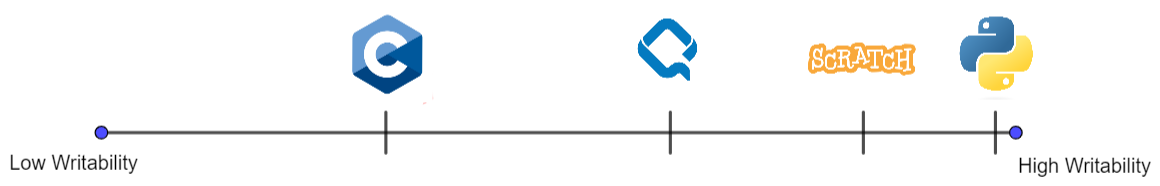
\includegraphics[width=0.9\textwidth]{Files/Billeder: Analyse/Writability.png}
    \end{center}
    \caption{The programming languages C, Python, Quorum, and Scratch placed on a scale showing writability. The red arrow indicates an assumption of where \lang lies on the scale}
    \label{writability}
\end{figure}

\subsubsection{Comparing reliability}
Scratch does not have exception handling and is dynamically typed. If the programmer decides to set the value of a variable equal to two strings added together, no error is displayed, and instead, the value becomes 0. This makes Scratch less reliable, as the programmer is not warned about unwanted behavior. Scratch does have restricted aliasing making it slightly more reliable.\\

Python is dynamically and strongly typed, and is able to for example interpret strings to numbers and vice versa, however, the programmer can get unwanted behavior when letting Python do automatic type conversion. Python still allows for explicit type conversion though. This gives Python lower reliability than other languages on the list, but higher reliability than Scratch.\\

In C the programmer does not have access to exception handling, but C is statically typed making it more reliable than Python and Scratch. C has limited support for restricted aliasing, but with its focus on using pointers, it does have aliasing.\\

Quorum provides exception handling for the programmer and is statically typed. This makes Quorum more reliable. Quorum is also placed more left than C because despite it having aliasing like C, C focuses a lot on pointers which is not included in Quorum. \\

\lang is being placed between C and Quorum on this scale. This is because the language will not include exception handling, as this is not a necessary tool for beginners in programming. To avoid type conversion errors, the language will be statically typed and have type-checking in order to avoid confusion for new programmers. The language will have limited or restricted aliasing, as references are a more advanced concept.

\begin{figure}[H] 
    \begin{center}
        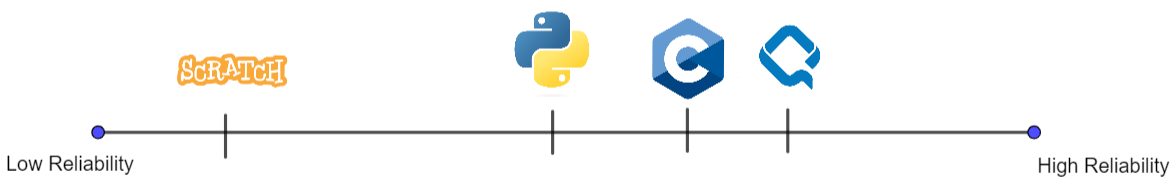
\includegraphics[width=0.9\textwidth]{Files/Billeder: Analyse/Reliability.png}
    \end{center}
    \caption{The programming languages C, Python, Quorum, and Scratch placed on a scale showing reliability. The red arrow indicates an assumption of where \lang lies on the scale}
    \label{reliability}
\end{figure}
\end{comment}

\section{Summary}

To summarize, The languages above are compared based on their ability to be understood by beginners, written in a straightforward way, and produce the desired output without errors. The analysis shows that C has the lowest readability and writability, while Python has high expressivity, which makes it easier to write code. Quorum focuses on readability over writability, making it more beginner-friendly. Scratch is also beginner-friendly but has limited expressivity. In terms of reliability, C is statically typed, which makes it more reliable than Python and Scratch. Quorum provides exception handling and is also statically typed, making it more reliable than C. C lacks exception handling, making it less reliable than Quorum.

\section{Problem statement} \label{problemstatement}
%From the analysis, a gap between the current existing languages can be seen. Based on the fact that many beginner programmers find it difficult to transition from any block-based language to some of the industry standard languages, a need for a language that can be used to handle this transition is needed. \\

%\noindent From this the following problem statement can be derived. \\ \\
%\noindent \textit{Explain and display a text-based programming language, which is aimed towards transitioning beginner programmers into using industry standard programming languages.}

From the analysis, a vacancy between the existing languages can be seen. As a beginner programmer, there are several ways to learn to program. Learning to program in a block-based language is widely used and tends to be a positive way to evolve computational thinking and be introduced to programming. But despite this, beginner programmers find it difficult to transition from a block-based language to some of the industry standard languages. The introduction to a text-based programming language is challenging and requires persistence. \\
Based on the analysis and comparison of the four different languages there are different pros and cons seen from a beginner's perspective. By the conclusion of the analysis, the goal of our language is a beginner-friendly text-based language that is developed to introduce beginner programmers to the basic and important concepts in programming is needed. \\

From this, the following problem statement can be derived.

\begin{center}
    \textit{How can a text-based programming language be developed for beginner programmers, using readable concepts from block-based languages, while focusing on facilitating the transition to programming languages used in the industry?}
\end{center}

A list of requirements has been made in order to successfully be able to say, that the problem statement has been solved. The list has been made in chronological order, and the details, importance, and use will be presented throughout the report.

% \begin{itemize}
% %  \item Analyze beginner programmers.
%   \item Define language criteria for \lang.
% %  \item Explain the programming paradigm of \lang.
% %  \item Create a MoSCoW requirement table.
%   \item Create and explain the Context-Free Grammar (CFG) for \lang.
%   \item The creation of a lexer and parser.
%   \item Define semantics for \lang.
%   \item Abstract Syntax Tree (AST) design for \lang.
%   \item Definition of scope rules.
%   \item Successful type checking and symbol table creation
%   \item Successful code generation
%   \item Evaluate the extent to which the language criteria were implemented.
% %  \item Show how the Syntax analysis, the Contextual analysis, and the code generation have been implemented.
%   \item Testing of \lang, including unit testing, integration testing, and acceptance testing.
% %  \item Evidence in the form of tests, to support the claim that our language helps provide the beginner programmer with a better transition from our language to an industry-standard language.
%   \item A discussion to reflect on the process.
%  % \item Sørge for at nævne alle at vil opfylde alle punkter i studieordningen.
% \end{itemize}

\begin{itemize}
%  \item Analyze beginner programmers.
  \item Define language criteria.
%  \item Explain the programming paradigm of \lang.
%  \item Create a MoSCoW requirement table.
  \item Create a Context-Free Grammar (CFG).
  \item Define semantics.
  \item Define the scope rules.
  \item Design Abstract Syntax Tree (AST).
  \item Create a lexer and parser.
  \item Build symbol table and handle type checking.
  \item Successful code generation
%  \item Show how the Syntax analysis, the Contextual analysis, and the code generation have been implemented.
  \item Testing of \lang, including unit testing, integration testing, and acceptance testing.
%  \item Evidence in the form of tests, to support the claim that our language helps provide the beginner programmer with a better transition from our language to an industry-standard language.
\end{itemize}